\documentclass[a4paper,10pt]{article}
\usepackage[utf8]{inputenc}
\usepackage[T1]{fontenc}
\usepackage[french]{babel}
\usepackage[normalem]{ulem}
\usepackage{geometry}
\usepackage{lmodern}
\usepackage{graphicx}
% \usepackage{setspace}
% \usepackage{titlesec}
\usepackage{geometry}
\usepackage{placeins}
% \usepackage{epsfig}
% \usepackage{hyperref}
% \usepackage{url}
% \usepackage{cite}
% \usepackage{listings}
% \usepackage{xcolor}


\geometry{top=3cm, bottom=3cm, left=2cm, right=2cm}

\title{Rapport\\Architecture Logicielle\\Jeu 2D autour d'un framework\\Année 2015/2016 }
\author{Raphaël Jorel, Antoine Laulan}



\begin{document}


\begin{figure}
    \begin{center}
    
\includegraphics[scale=0.7]{images/logo-bdx.pdf}
    \end{center}
\end{figure}
\maketitle




\newpage
\section{Introduction }
Notre jeu a été produit dans le cadre de l'UE architecture logicielle. Le but étant de créer un jeu à l'aide
d'un framework fourni et cela sans modifier celui-ci.
Dans ce rapport nous présenterons notre jeu et nous fournirons une critique du \textit{framework} utilisé. \\

Comme le sujet était libre, nous avons choisi de recréer une copie simplifiée du célèbre jeu \textit{Breakout}.
Simple en apparence, mais qui nous aura tout de même donné du fil à retordre sur certains aspects
que nous ne soupconnions pas. Nous dédierons une partie à l'explication de ces problèmes rencontrés.


\section{Firewall Breaker}
\subsection{Présentation}
    Tout d'abord, une petite capture d'écran afin d'apprécier le rendu du jeu et des \textit{assets} qui ont été
    utilisés  :

\FloatBarrier
		\begin{figure}[!h]
    		\begin{center}
	   	  	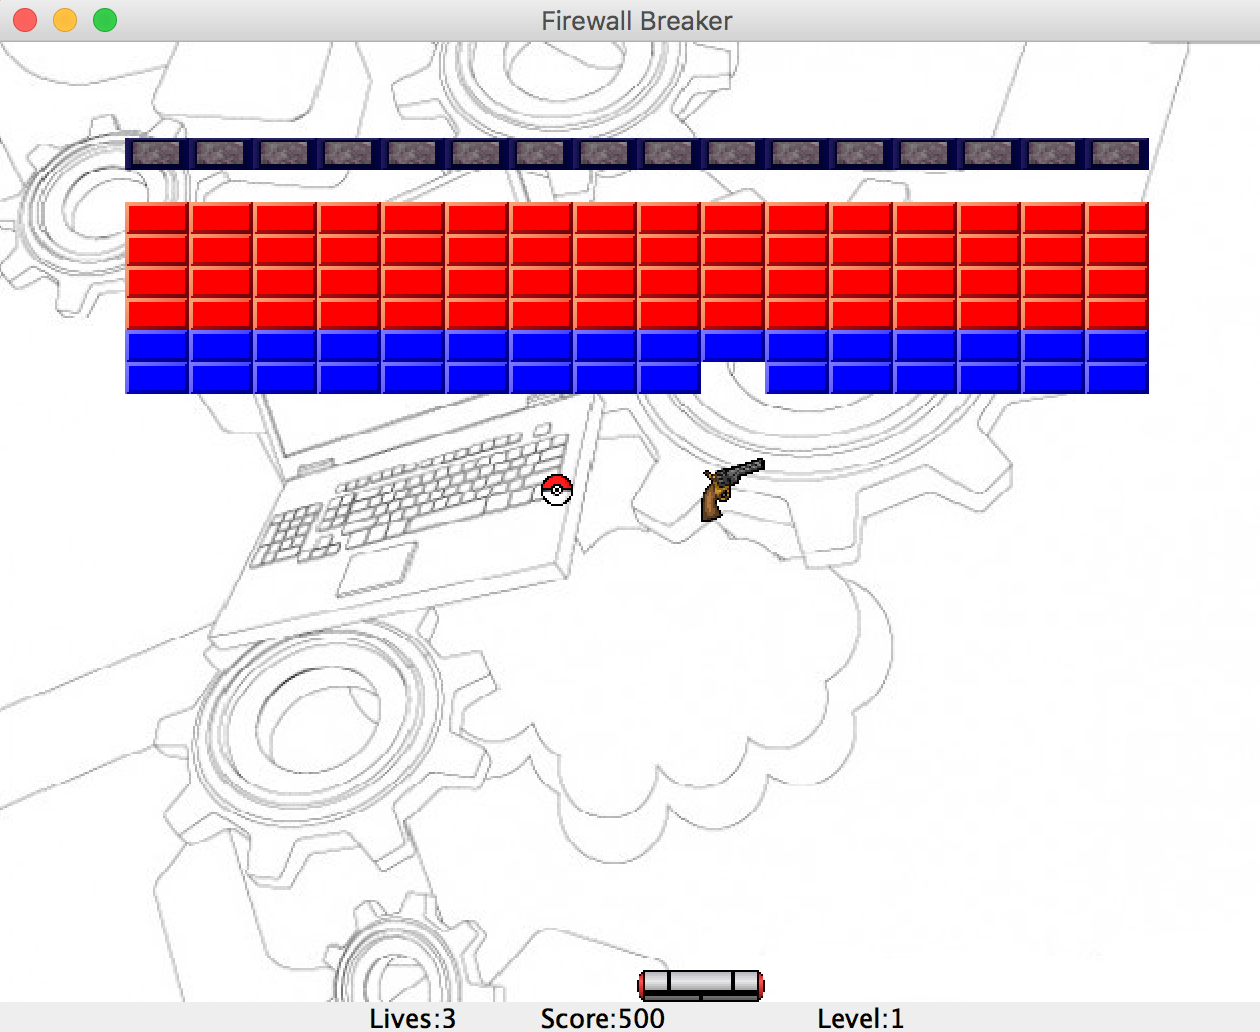
\includegraphics[scale= 0.5]{images/gameView.png}
          	\caption{Vue du jeu}
    		\end{center}
		\end{figure}
\FloatBarrier

Le joueur contrôle une palette et doit, en faisant rebondir la balle, détruire les briques pour gagner.
Pour se faire, il peut être aidé de divers bonus et briques spéciales. La partie s'arrête lorsque le joueur
a détruit toutes les briques qui peuvent l'être, ou lorsque celui-ci n'a plus de vie.

\subsection{Fonctionnalités du jeu}
    \subsubsection{Le joueur}
        Le joueur ne peut faire que deux choses : aller à droite ou à gauche. Il doit rattraper la balle
        qui se déplace pour la relancer dans le jeu et ainsi casser les briques. Comme sus-dit, il pourra
        être aidé par différents bonus, et ainsi augmenter sa capacité de destruction.

	\newpage
    \subsubsection{La balle}
        La balle se déplace et rebondit sur les briques, les murs (invisibles sur les côtés) et le joueur.
        Ses rebonds gardent les mêmes angles lorsqu'elle rebondit sur les murs et les briques, mais suivant
        l'endroit où elle touche le joueur, elle gagne ou perd en vitesse.

    \subsubsection{Les briques}
        Il y a quatre sortes de briques :
        \begin{itemize}
            \item les basiques : elles n'ont aucun effet particulier, mis à part le fait de rapporter des points
            lorsque la balle les détruit,
            \item les indestructibles : elles font barrage à la balle et ne peuvent être détruites,
            \item les briques de bonus : elles déclenchent l'apparition aléatoire de bonus lorsqu'elles sont détruites,
            \item les briques explosives : elles explosent lorsqu'elles rentrent en contact avec la balle et cassent
            toutes les briques situées autour d'elles
                    et ceci dans un rayon de taille aléatoire. \\
        \end{itemize}

        Lorsque toutes les briques sont cassées, le niveau est terminé. Toutes les briques destructibles
        ne nécessitent qu'un seul coup pour être détruites.

    \subsubsection{Les bonus}
        Afin de varier un peu le jeu et de coller un peu plus à l'esprit d'un Breakout, nous avons donné la possibilité au joueur
        d'utiliser des bonus. Ceux-ci ont uniquement un effet "positif" sur la partie du joueur. Voici la liste des bonus mis
        à la disposition de ce dernier :
        \begin{itemize}
            \item \textbf{Vie} : représenté par un coeur, caractérisé par le rajout d'une vie supplémentaire,
            \item \textbf{Mitraillette} : représenté par un pistolet et caractérisé par le tir d'une salve (limitée dans le temps)
            de balles depuis la palette du joueur en direction des briques,
            \item \textbf{Bombes} : représenté par une bombe. Ce bonus à pour effet de transformer une brique restante
            en brique explosive et de la faire exploser. L'explosion a le comportement d'une brique explosive classique.
            \item \textbf{Fireball} : représenté par une boule de feu. Il provoque un changement d'état temporaire de la balle
            qui ne 	rebondit alors plus sur les briques mais passe à travers tout à l'exception des briques indestructibles. \\
        \end{itemize}

        Chacun de ces bonus est associé à une probabilité, ainsi  par exemple le bonus de vie supplémentaire a moins
        de chance d'apparaître que les autres, car le nombre de vies est un élément cruxial à prendre
        en compte, et que nous ne souhaitons pas que le jeu soit trop facile, cela va de soit.

    \subsubsection{Gestion des parties}

       	\paragraph{Nouvelle partie.} Il est toujours agréable de pouvoir recommencer une partie, sans etre obligé de relancer un
        programme. Pour cela, la fonctionnalité \textit{new (game)} a été apportée, en plus de la
        possibilité de quitter. Cependant, il est impossible de suspendre une partie et de la reprendre.
        Il faut donc que vous soyez vraiment sûr de ne pas être dérangé et de n'avoir rien besoin de faire pendant vos parties.

		\paragraph{Charger un niveau.} L'utilisateur à la possiblité de charger ses propres niveaux de jeu. Des détails sur
		cette fonctionnalité seront apportés dans la partie dédiée à l'implémentation.

        \paragraph{Enchainement des niveaux. } Lorsque le joueur perd le jeu ou le gagne, il en est informé par un message approprié. Cependant, le jeu démarre
        directement sans attente et la transition entre niveau est directe. Soyez concentré car il faudra
        se resituer très vite lorsqu'un niveau sera terminé et que le suivant apparaîtra.

	\subsubsection{Fonctionnalités futures}
		Comme tout jeu récent nous proposerons des DLC payants (contenu téléchargeable) aux utilisateurs. Ils auront pour but
		d'augmenter le nombre de type de brique et d'ajouter de nouveaux bonus encore plus dévastateurs..

\subsection{Architecture}
    Un bon jeu implique une bonne architecture. L'inverse est quant à lui moins évident...
	Nous allons dans cette partie vous présenter l'architecture logicielle de notre jeu. Ceci sera fait à l'aide de
	diagrammes de classes.
	Nous mettrons en évidence les connexions entre nos classes et les classes du \textit{framework}.

% 	\newpage
	\subsubsection{Diagrammes de classe}

		\FloatBarrier
		\begin{figure}[!h]
    		\begin{center}
	  	  	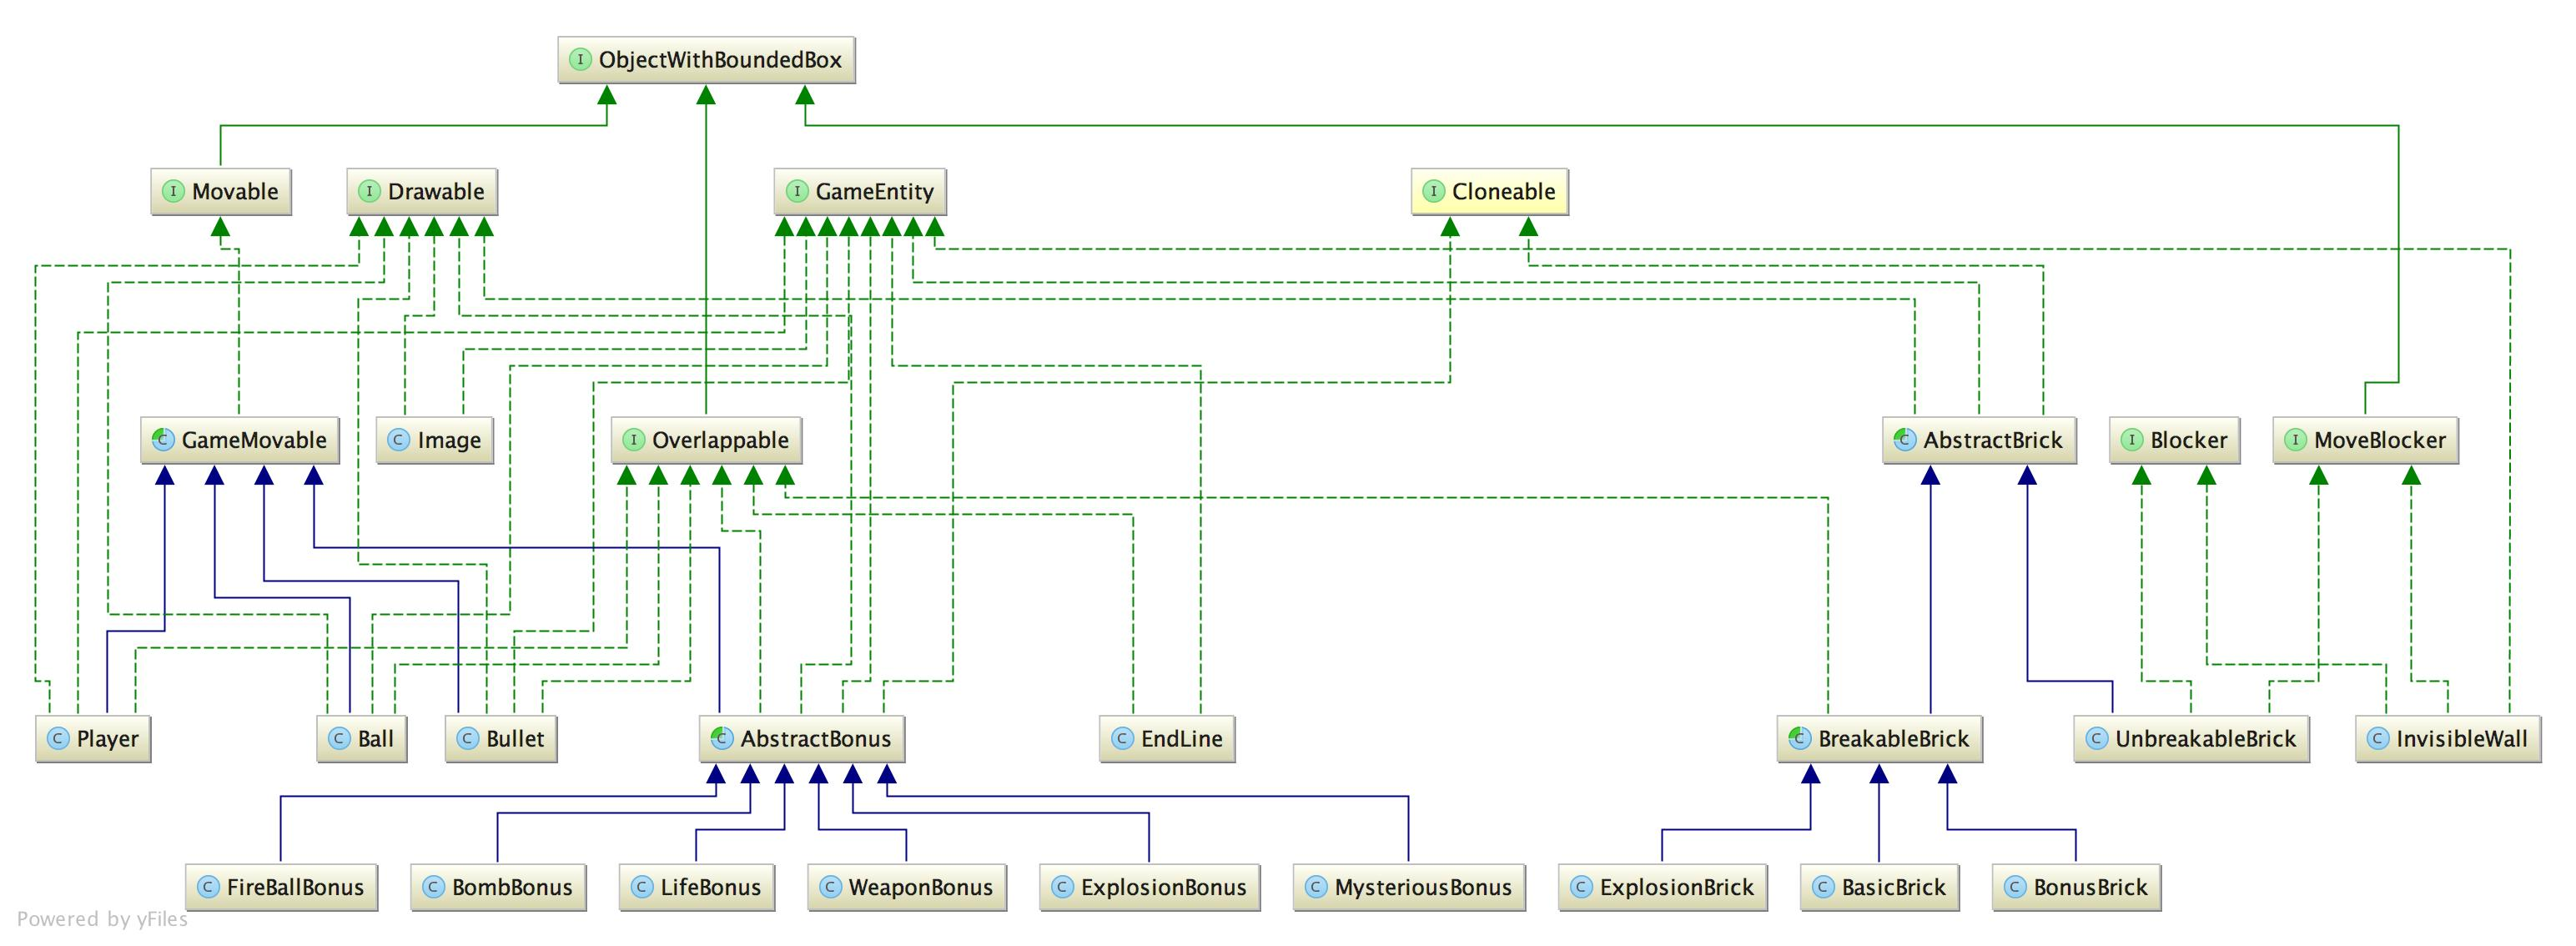
\includegraphics[scale=0.17]{images/whiteEntityDiagram.jpg}
          	\caption{Diagramme de classe des entités}
    		\end{center}
		\end{figure}
		\FloatBarrier


 		\FloatBarrier
 		\begin{figure}[!h]
     		\begin{center}
 	  	  	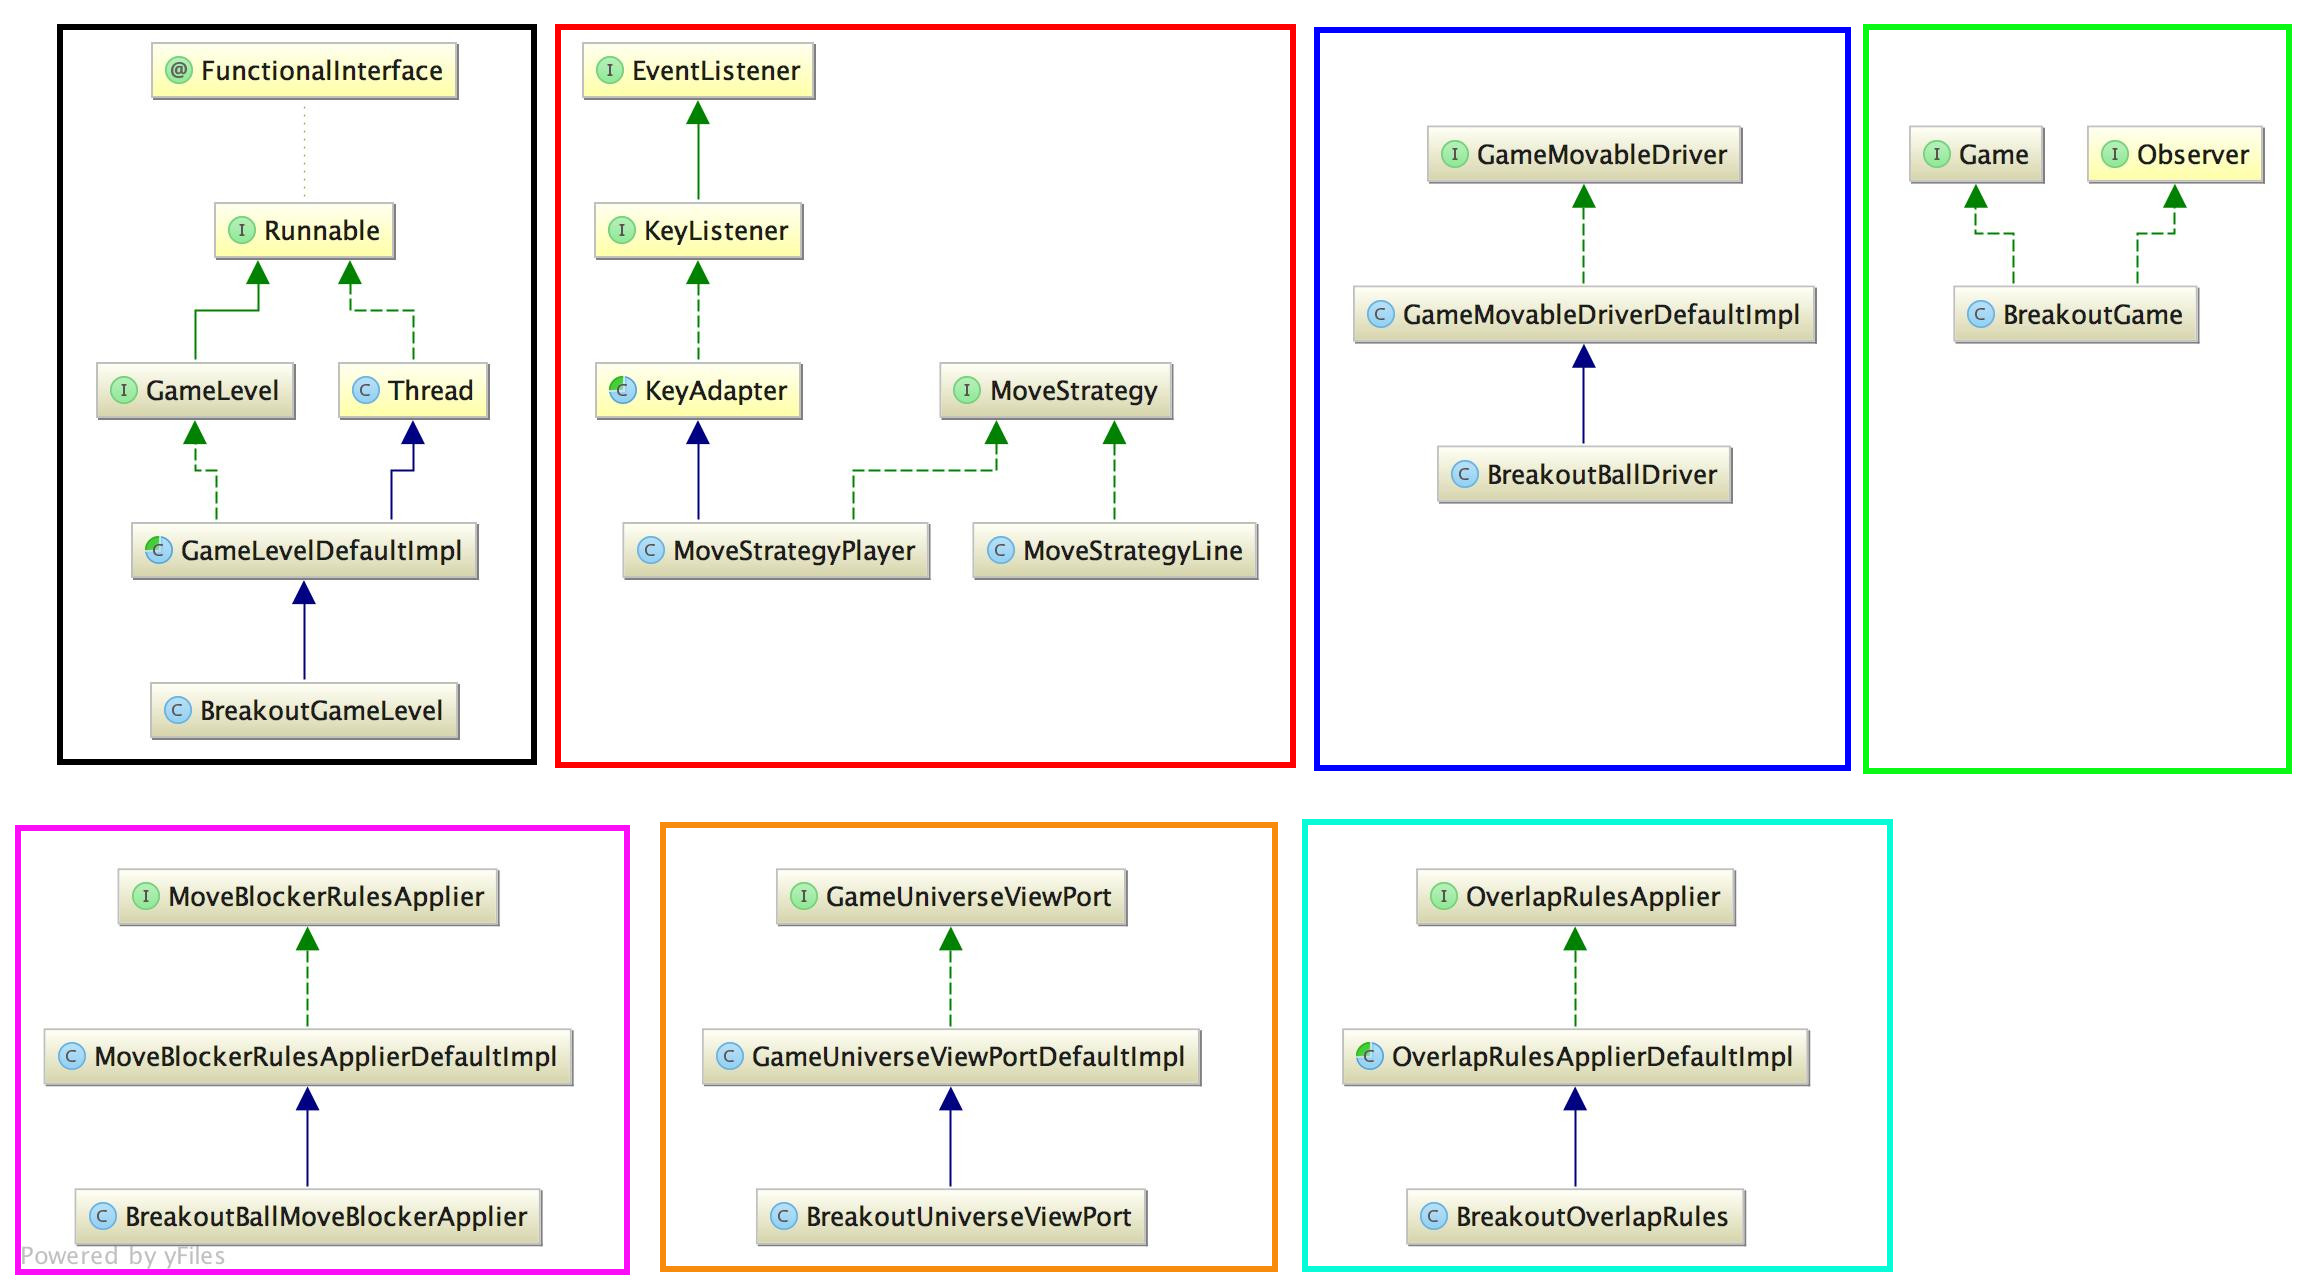
\includegraphics[scale=0.2]{images/whiteSeveralDiagram.jpg}
           	\caption{Multi diagramme de classe}
     		\end{center}
 		\end{figure}
 		\FloatBarrier
 		\paragraph{Description :}
 		Plusieurs classes forment de petits diagrammes de classes. Nous les avons regroupés dans une seule est même image.
 		Pour les différencier
 		nous avons utilisé un code couleur. Ce code couleur est détaillé dans la liste suivante : \\
 		\begin{itemize}
 		\item noir : gestion des niveaux du jeu,
 		\item rouge : stratégie de déplacement du joueur,
 		\item bleu : \textit{driver} de la balle,
 		\item vert : gestion de la fenêtre IHM du jeu,
 		\item rose : \textit{move blockers} pour la balle et le joueur,
 		\item orange : gestion du fond d'écran,
 		\item bleu ciel : gestion des \textit{overlappables}.
 		\end{itemize}


\subsection{Implémentation}
    Après cette présentation des fonctionnalités et de l'architecture du jeu, nous allons
    parler de son implémentation et donc du travail qui a été effectué.

    \subsubsection{Les niveaux}

        \paragraph{Description.} Afin de ne pas avoir à écrire statiquement la configuration des briques d'un niveau, nous avons
        utilisé des fichiers externes, au format \textit{.txt}, pour le faire. Chaque type de brique est représentée par un numéro.
        Théoriquement, il est possible d'avoir un nombre de brique en largeur et en hauteur aussi grand qu'on le souhaite.
        Il faut préciser cela dans au début du fichier de description, mais pour des raisons de jouabilité, il
        est recommandé de se limiter à des grilles de 16x16. Ainsi, la balle a toujours la place de bouger entre les murs
        extérieurs et les briques. \\

        Pour éviter d'instancier chaque brique une à une, nous nous sommes servis du \textit{design pattern prototype},
        permettant d'avoir les briques de bases dans un tableau et ensuite de les cloner en fonction du
        fichier de description.

        \paragraph{Fichiers de description.}
        Comme expliqué dans les fonctionnalités, il est possible de charger ces propres niveaux. Pour cela, il suffit
        d'écrire un fichier de description, comme ceux qui sont utilisés pour les niveaux pré-définis. \\
        Un fichier de description commence par la valeur du nombre de briques en largeur, puis celle en hauteur (16 16
        en général). Ensuite, il suffit de préciser les identifiants des briques dans l'ordre souhaité. Ces identifiants
        sont :
        \begin{itemize}
            \item $0$ pour une espace vide,
            \item $1$ pour une brique indestructibles,
            \item $2$ pour une brique normale,
            \item $3$ pour une brique de bonus,
            \item $4$ pour une brique explosive.
        \end{itemize}


    \subsubsection{Stratégies de déplacement}
        Les stratégies permettent de définir comment un objet va se déplacer. Pour notre jeu, nous n'avons eu besoin
        que de deux stratégies  : celle du joueur et celle des autres entités. \\ Les autres entités
        se déplacent verticalement, vers le bas pour les bonus et vers le haut pour les balles de pistolet. La balle, quant
        à elle décrit plutôt des diagonales. Mais toutes ces entités se déplacent en décrivant des lignes droites.
        Le joueur quant à lui bouge suivant l'action de l'utilisateur sur le clavier. Son déplacement est uniquement horizontal.

    \subsubsection{Fenêtre de jeu}
        En s'inspirant de l'exemple d'utilisateur du \textit{framework}, nous avons créé une fenêtre de jeu semblable,
        mais évidemment plus appropriée au jeu de \textit{Breakout}. \\
%         La possibilité de recommencer une partie et de la quitter
%         font parties des deux seules fonctionnalités de la fenêtre d'affichage. \\

        Afin de gérer la fonction \textit{new}, nous avons remanié l'exemple donné pour lui permettre de fonctionner
        correctement. Nous gérons les niveaux dans une file de \textit{threads} qui attendent d'être lancés. Lorsque la file
        est vide, le jeu se bloque et attend. Une fois que le joueur a fait \textit{new}, la file de \textit{threads} est
        à nouveau remplie, et ces derniers peuvent être relancés. Si jamais l'utilisateur fait \textit{new} avant
        la fin du jeu, le \textit{thread} courant est arrêté, pour pouvoir repartir sur un jeu ``neuf''. \\

        C'est également la fenetre de jeu qui gère les messages de fin de partie. Elle les affiche à l'utilisateur
        l'informant de sa réussite ou de son échec dans une fenêtre de dialogue. Pour recommencer une partie, il
        est nécessaire de fermer cette fenêtre additionnelle. \\

        Enfin, nous avons pensé à faire un \textit{memento} pour pouvoir sauvegarder l'état du jeu et pouvoir le
        restaurer à la demande du joueur. Mais nous avons arreté de poursuivre son implémentation quand nous avons
        compris que, pour notre jeu, cela demandait de retenir trop de données éparpillées dans le jeu. Il aurait
        fallu alourdir les classes existantes avec de nouvelles fonctions, pour une fonctionnalité qui finalement
        nous semblait peu utile.

    \subsubsection{Les rebonds}
        Une mauvaise impression sur les rebonds peut rebuter quelque peu l'utilisateur. Nous approfondirons
        cet aspect dans les difficultés rencontrées.

        \paragraph{Entités indestructibles.}
        Nous effectuons les rebonds de façon
        différentes sur les briques destructibles et indestructibles, car ces dernières sont considérées comme \textit{blockers}. \\
        Lorsque la balle est bloquée par l'une d'elle, nous proposons au \textit{driver} de la balle des possibilités
        de stratégies à essayer afin de choisir celle qui est applicable pour que la balle puisse continuer à se déplacer.

		\subparagraph{Calcul du point de collision.}
            Les murs et les briques indestructibles sont des \textit{blockers}, c'est-à-dire que le système calcule avant de
            déplacer les entités mobiles (comme la balle) si ces dernières rentrent en collision avec les \textit{blockers}.
            Et si c'est le cas, l'entité ne sera pas déplacée. Ceci pose un problème lorsque la balle est trop rapide. En
            effet, le système considérera qu'une entité ne pourra pas être déplacée, alors qu'en raison de sa grande vitesse,
            elle ne sera pas collée à un mur ou une brique incassable. Pour rémédier au problème, il suffit de vérifier si
            la balle est effectivement collée ou pas, et ensuite calculer le point de collision si besoin.
            Comme nous ne modifions la vitesse que sur l'axe des abscisses, ce calcul n'est pas effectué sur celui des
            ordonnées.

        \paragraph{Entités destructibles.}
		Cependant la façon de faire avec les entités destructibles est différente. Les briques ne sont plus des \textit{blockers}
		mais des \textit{overlappables}. Ceci implique que les entités peuvent se "chevaucher" et que donc, si l'on veut que les
		briques cassables aient le comportement désiré, à savoir modifier la trajectoire de la balle et être destructible, il faut
		calculer le point d'impact entre les deux entités. Ce calcul est important car c'est lui qui permettra de définir
		quand la balle rencontre une brique et quand elle doit modifier sa trajectoire.

		\subparagraph{Calcul du point de collision.}
		Les briques sont représentées par des rectangles et la balle par un carré.
		Afin de trouver le bon point de collision et ainsi faire la bonne modification de trajectoire nous avons procédé comme expliqué dans la liste
		suivante :
		\begin{itemize}
		\item calcul de la position de la brique à l'aide des quatre points qui la représente,
		\item calcul des points de collision de la balle, à savoir le milieu de chacun des côtés du carré qui contient la balle,
		\item comparaison des positions entre les côtés du rectangle et les points de collisions de la balle,
		\item si un point de collision dépasse le côté correspondant du rectangle, la trajectoire est changée. \\
		\end{itemize}
		Les correspondances sont les suivantes :
		\begin{itemize}
		\item le haut de la balle avec le côté bas du rectangle,
		\item le bas de la balle avec le côté haut du rectangle,
		\item la gauche de la balle avec le côté droit du rectangle,
		\item la droite de la balle avec le côté gauche du rectangle. \\
		\end{itemize}
		Cependant cette approche a apporté quelques problèmes de collisions justement. Nous approfondirons ce point
		dans la partie dédiée aux difficultés rencontrées. \\

        En ce qui concerne les murs, nous ne faisons qu'inverser la vitesse sur l'axe des ordonnées ou des abscisses suivant
        que le mur rencontré est horizontal ou non.


    \subsubsection{Briques}
        Les briques sont toutes issues de la meme classe abstraite. Cette classe gère quasiment tout, les briques ne font
        que définir des types qui seront utiles pour identifier les entités qui se touchent. Principalement, elles
        précisent leur image qui sera affichée pour les identifier à l'écran. \\

        Nous souhaitions alléger la mémoire utilisée par les briques. En effet, chaque brique a sa propre image, or
        il n'y a que quatre type de briques. C'est pourquoi nous avons pensé à stocker ces quatres images dans un
        tableau statique. Lors qu'une brique doit être affichée, elle ne fait que préciser l'indice de l'image
        dans le tableau statique. Mais le gain n'était pas assez important pour justifier la mise en place de
        ce système assez lourd et peu lisibible. Cependant, nous avons gardé la classe, car elle pourrait être
        utilisée si jamais les images des briques devenaient vraiment très lourdes.

    \subsubsection{Bonus}
        Les bonus n'ont pas été la partie la plus dure à implémenter et penser, bien qu'elle nous ait demandé un peu
        d'imagination. Le plus dur a finalement été de comprendre bien le \textit{framework} pour savoir
        comment arriver à nos fins. \\

        Comme pour les briques, il y a une classe abstraite à la base de tous les bonus. Les classes concrètes
        sont là surtout pour définir des types.

        \begin{itemize}
            \item \textbf{Vie :}
                Le bonus de vie est extremement simple, il nous a suffit d'incrémenter le compteur de vie du joueur
                pour le mettre en place.

            \item \textbf{Mitraillette :}
                Peut-être celui qui a demandé le plus de recherche pour être mis en place, les salves sont tirées
                si le joueur est toujours sous l'effet du bonus. Cet effet est appliqué avant que les entités
                ne vérifient qu'elles se touchent.

            \item \textbf{Bombes :}
                Pour cet effet, il a d'abord fallu récupérer toutes les entités présentes dans le jeu et trier
                pour ne garder que les briques destructibles. Ensuite, une brique est tirée aléatoirement pour exploser.

            \item \textbf{Fireball :}
                Ce bonus n'impose plus de contraintes sur la balle. Il est mis en place en vérifiant que le joueur
                est toujours sous l'effet du bonus et en n'appliquant pas le changement de direction de la balle lorsque
                cette dernière entre en collision avec les briques destructibles.
        \end{itemize}




\subsection{Limites du jeu et difficultés rencontrées}


Même les grands jeux ont des limites, prenez par exemple \textit{Assassin's Creed Unity}... quoique dans ce cas,
il s'agisse plutôt de bugs.

\paragraph{Les collisions.}
La gestion des collisions n'a pas été chose simple, aussi il est assez remarquable par moment que la balle
ne rebondit pas comme souhaité. Cela vient principalement du \textit{framework} qui permet difficilement d'avoir
conscience du contexte de la balle. De plus, ce dernier permet que la balle touche plusieurs briques à la fois,
ce qui peut entraîner des comportements inattendus, vu que la trajectoire de la balle est modifiée plusieurs fois. \\

Rentre également en ligne de compte la vitesse de la balle. C'est-à-dire que si la balle est trop rapide alors durant
le temps qui s'écoule entre deux \textit{laps} (itérations de jeu), la balle s'est déplacée à ``l'interieur'' d'une brique.
En d'autres termes, les
deux \textit{overlappables} se chevauchent un peu trop. Et par conséquent, plusieurs
points de collision de la balle ont dépassé leur côté. De ce fait, c'est l'ordre des \textit{if} et \textit{else if} qui dicte
le choix de la nouvelle trajectoire à prendre pour la balle. Or il peut arriver que ce choix soit erroné par rapport à la
trajectoire initiale de la balle.\\
Concrètement les rebonds sur le dessus et sur le dessous des briques sont à peu près corrects tandis que ceux sur
les côtés droit et gauche sont faussés. En inversant l'ordre des \textit{if} / \textit{else if} il est possible de rendre
ces rebonds cohérents mais cela a pour conséquence de fausser ceux du dessus / dessous. \\

Autre problème remarqué, lorsque la balle se retrouvent à la fois bloquée par une brique indestructibles (type \textit{blocker})
et en collision avec une autre brique (type \textit{overlappable}), il y a des comportement inattendus, comme le blocage
de la balle dans le \textit{blocker} par exemple.

\paragraph{Les images d'explosion.}
Pour des raisons qui nous échappent également, l'image des explosions ne disparaît pas certaines fois. Il est possible
que ce soit dû à des problèmes de collisions multiples d'une brique avec une bombe et une autre élément du jeu (les
balles tirées par exemple). Ceci dit, le problème semble n'apparaître que très rarement.


\section{Critiques du framework }
    Passons maintenant aux critiques du \textit{framework}. "La critique est aisée mais l'art est difficile" \textit{P.Destouches}.
    Il est toujours plus facile de critiquer que de faire, donc comme nous avons fait, place à la critique. Nous tenterons
    cependant d'être les plus magnanimes possible, cela va de soit.

    \subsection{Nom des classes}
        Mention spéciale aux noms des classes fort longs parfois. Bien que cela explicite peut-etre le rôle
        de chaque classe, il est parfois bien compliqué de s'y retrouver, et de comprendre le fonctionnement,
        car les noms ne différent pas de beaucoup par moment et il est fréquent de les confondre.
        De plus, les suffixes \textit{DefaultImpl} alourdissent les noms et sont peut-être inutiles.

    \subsection{Introspection}
       	 Nous avons appris que l'introspection faisait perdre en performances. Et pourtant, le \textit{framework} s'en sert
        pour faire appel aux fonctions de gestion des collisions. Ceci permet d'ajouter les règles de collision
        qui nous intéressent, mais n'oublions pas que les performances en patissent. De plus, cette technique est
        utilisée à deux endroits dans le code, et cela est appliqué à chaque itération du jeu (\textit{lap}).

    \subsection{Image de fond}
        Pour créer un niveau, il est nécessaire d'avoir un \textit{viewport}, ce que le système fournit. Ce qui est
        par contre assez difficile à comprendre, c'est pourquoi la classe gérant \textit{viewport} par défaut
        comporte une méthode qui permet de modifier l'image de fond, alors que finalement la méthode permettant de connaître
        cette image ne fait que renvoyer une chemin vers un fichier ? Et cela écrit en dur en plus ! Conclusion, une classe
        fille seulement à cause d'une méthode qui fait un travail assez inattendu.

    \subsection{Gestion des niveaux}
        Pourquoi avoir géré les niveaux comme des threads ? Bonne question. Une fois qu'ils sont lancés il est impossible de les
        relancer, impossible de les cloner et la gestion devient compliquée, etc.. Nous supposons que cela est pour permettre
        à l'\textit{EventDispatcher} de faire son travail avec l'interface du jeu. Cependant le travail pour gérer
        les niveaux est bien plus complexe. \\
        D'ailleurs, l'exemple donné (le \textit{Pac Man}) ne gère pas bien cela. Il suffit de rajouter un niveau au jeu
        pour se rendre compte que lorsque l'on fait un \textit{new} le jeu lance
        deux niveaux en même temps, en les superposant. Mais cela vient d'une boucle \textit{foreach} sur les \textit{threads} et donc
        la liste de niveau se retrouve parcourue à deux endroits différents. De plus, le \textit{Pac Man} ne gère
        pas le \textit{new} lorsque le jeu est terminé. Et ceci est normal, car un \textit{thread} ne peut être
        relancé. Pour pallier au problème, nous ne donnons que les chemins vers les fichiers de définition des
        niveaux et nous recréons des \textit{threads} à chaque \textit{new}.

    \subsection{La facilité a un coût}
        Le \textit{framework} permet une mise en place rapide de jeux, et fournit les éléments nécessaires pour
        que cela soit jouable. Mais cette facilité est compensée par le fait qu'il n'est pas évident (à moins
        de réécrire certaines classes) de faire des choses très poussées. En effet, comme évoqué dans la partie
        implétementation, le système considère les collisions avec les \textit{blockers} de façon très basique.
        Il n'y pas de vérifications qui permettrait d'approcher les \textit{blockers} de façon plus
        fine. C'est d'ailleurs pour cela que nous avons dû calculer nous-même le point d'impact quand cela
        était nécessaire.

    \subsection{Une classe de gestion des collisions à rallonge}
        Sans aller jusqu'à dire qu'il faille toujours que les classes soit courtes pour être plus facilement
        réutilisables, et que donc les classes très longues sont à bannir, il y a peut-être
        des limites.
        Autant pour la classe gérant la fenêtre d'affichage, cela parait logique car il y a beaucoup
        de code pour mettre en place les éléments, autant des fois c'est évitable. Nous pointons du doigt ici la classe
        qui gére les collisions entre les entités \textit{overlappables}. La côté pratique, c'est que tout est au
        même endroit, celui qui l'est moins, c'est qu'avec quelques centaines de lignes de codes et des fonctions
        qui se nomment toutes \textit{overlapRule}, il n'est pas si évident de s'y retrouver.


\section{Conclusion}
    Pour conclure, nous pouvons dire que le projet a été tout de même fort agréable à réaliser, bien que la compréhension
    du \textit{framework} ne fut pas triviale et que cela a constitué notre principal frein.  \\
    Ceci dit, faire un jeu
    a vraiment été un plaisir, de par de son côté évidemment ludique... et ça change de faire des sites web avec des bases
    de données.


\end{document}
% \grid
